\documentclass[a4paper]{article}

\usepackage[english]{babel}
\usepackage[utf8]{inputenc}
\usepackage{amsmath}
\usepackage{graphicx}
\usepackage[colorinlistoftodos]{todonotes}
\usepackage{tikz}
\usetikzlibrary{arrows}

\tikzset{
  treenode/.style = {align=center, inner sep=0pt, text centered,
    font=\sffamily},
  arn_n/.style = {treenode, circle, white, font=\sffamily\bfseries, draw=black,
    fill=black, text width=1.5em},% arbre rouge noir, noeud noir
  arn_r/.style = {treenode, circle, red, draw=red, 
    text width=1.5em, very thick},% arbre rouge noir, noeud rouge
  arn_x/.style = {treenode, rectangle, draw=black,
    minimum width=0.5em, minimum height=1em}% arbre rouge noir, nil
}

\title{Rapport Recherche d'Informations Visuelles Structurées }

\author{Loic HERBELOT Sébastien PEREIRA}

\date{\today}

\begin{document}
\maketitle

\begin{abstract}
Dans ces TME nous allons nous intéresser au paradigme d'apprentissage structuré appliqué à différentes problématiques de recherche d'informations visuelles. On instanciera dans un premier temps ce problème pour résoudre des tâches de classification d'images puis dans un second temps pour résoudre un problème de ranking renvoyant les images qui correspondent à la recherche de l'utilisateur.
\end{abstract}

\section{Introduction}
Contrairement à la régression où notre espace de sortie $Y$ est tel que $y \in \Re $   et à la classification où $Y$ est tel que $y \in {1, 2, 3, ..., C}$ (où C est le nombre de classes), l'apprentissage structuré définit un espace de sortie $Y$ où les $y$ sont des structures comme des arbres des graphes des ordonnancements etc.
\subsection{Formalisme}
Soit $X$ l'espace d'entrée et $Y$ l'espace de sortie structuré.
On définit une \textit{joint feature map} $\Psi(x,y)$ qui décrit le lien entre l'entrée $x$ et la sortie $y$ et une fonction de coût $\Delta(y,y')$ qui mesure la dissimilarité entre notre prédiction et la vérité terrain.
Le problème d'apprentissage revient à trouver un modèle linéaire qui donne un score à chaque paire $(x,y)$, le score est définit par $<w, \Psi(x,y)>$
La prédiction du modèle est de la forme :
\begin{equation}
\hat{y}(x,w) = \arg\max_{y \in Y} <w, \Psi(x,y)>
\end{equation}

Le problème d'apprentissage s'écrit :
\begin{equation}
\min_{w} \frac{1}{2} {||w||}^2 + \frac{C}{n} \sum\limits_{i=1}^n \Delta(y_i, \hat{y})
\end{equation}
Ce problème d'optimisation étant NP difficile, on optimise une borne supérieure convexe et sous différentiable de $\Delta(y_i, \hat{y})$ définit par :
\begin{equation}
\max_{y \in Y} [\Delta(y_i, \hat{y}) + <\Psi(x_i,y),w>]  - <\Psi(x_i,y_i),w>
\end{equation}
Le problème d'optimisation devient donc :
\begin{equation}
\min_{w} \frac{1}{2} {||w||}^2 + \frac{C}{n} \sum\limits_{i=1}^n [ \max_{y \in Y} [\Delta(y_i, \hat{y}) + <\Psi(x_i,y),w>]  - <\Psi(x_i,y_i),w>]
\end{equation}

\subsection{Algorithme d'apprentissage}

\section{Apprentissage structuré Multi-classes et Hierarchique}
Dans cette première partie on s'intéresse à la classification d'images à partir d'un apprentissage supervisé, on s'intéressera à l'influence du choix de la fonction de coût sur les résultats obtenus.
\subsection{Classification Multi-classe}
Dans le cas d'un problème d'apprentissage structuré instancié pour les problèmes de classification multi-classe on définit la \textit{joint feature map} et la fonction de coût de la façon suivante : 
\begin{itemize}
\item $\Psi(x,y) = \begin{bmatrix}  0^d\\0^d\\...\\ \phi(x) \\...\\0^d\\0^d \end{bmatrix} $   
\item $\Delta(y,y') = \left\{
    \begin{array}{ll}
        1 & \mbox{si } y \neq y' \\
        0 & \mbox{sinon.}
    \end{array}
\right.$
\end{itemize}
Où $\phi(x)$ est la représentation des images sous forme de \textit{Bag of Words}
\begin{figure}
\centering
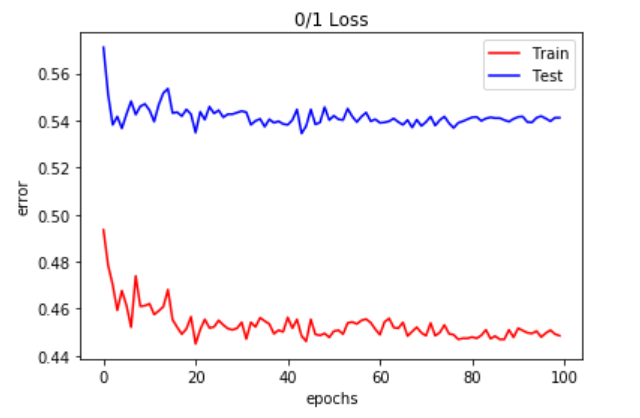
\includegraphics[width=0.75\textwidth]{error.png}
\caption{\label{fig:data} Évaluation de la 0/1 loss en train et en test sur 100 epochs.}
\end{figure}

\begin{figure}
\centering
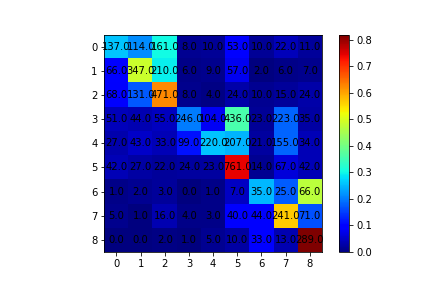
\includegraphics[width=1\textwidth]{confusion.png}
\caption{\label{fig:data} Matrice de confusion pour un modèle entrainé avec une 0/1 loss sur 100 epochs. 0 = taxi, 1 = ambulance, 2 = minivan, 3 = acoustic guitar, 4 = electric guitar, 5 = harp, 6 = wood frog, 7 = tree frog, 8 = european fire salamander}
\end{figure}
\subsection{Interprétation des résultats}
\begin{itemize}
\item la classe taxi (0) est très confondue avec la classe ambulance (1) et minivan (2)
\item la classe ambulance (1) est très confondu avec la classe minivan (2)
\item la classe minivan (2) est confondue avec la classe ambulance (1)
\item la classe acoustic guitar (3) est très confondue avec la classe electric guitar (4) et énormément confondue avec la classe harp (5)
\item la classe electric guitar (4) est très confondue avec la classe harp (5)
\item la classe harp (5) est très bien distinguée de toutes les autres classes
\item la classe wood grog (6) est beaucoup confondue avec la classe tree grog (7) et énormément confondue avec la classe european fire salamander (8)
\item la classe tree grog (7) est un peu confondue avec la classe european fire salamander (8)
\item la classe european fire salamander (8) est très bien distinguée de toutes les autres classes
\end{itemize}
\textbf{Conclusion} : on remarque qu'il existe 3 catégories sémantiques dans nos 9 classes, la première catégorie sémantique rassemble des véhicules (taxi, ambulance et minivan) la deuxième catégorie sémantique rassemble des instruments à cordes (guitare acoustique, guitare electrique et harpe) enfin la troisième catégorie sémantique rassemble des amphibiens (grenouille des bois, grenouille arboricole et salamandre). De plus on voit d'après la matrice de confusion que la grande majorité des erreurs de notre modèle provient de confusions au sein d'une même catégorie sémantique mises à part deux exceptions (harpe et salamandre), on peut donc en conclure que notre modèle n'arrivent pas à capter les différences entre les données provenant d'une même catégorie sémantique.

\subsection{Classification Hierarchique}
Dans le cas d'un problème d'apprentissage structuré instancié pour les problèmes de classification hierarchique on garde la \textit{joint feature map} précédente et on définit une fonction de coût de la façon suivante : 
\begin{itemize}   
\item $\Delta(y,y') = \left\{
    \begin{array}{ll}
        1 - \textit{Similarité}(y,y') & \mbox{si } y \neq y' \\
        0 & \mbox{sinon.}
    \end{array}
\right.$
\end{itemize}
Où la similarité est définit par une distance dans un arbre par exemple de la façon suivante (les noeuds désignent les similarités et les feuilles les classes) :
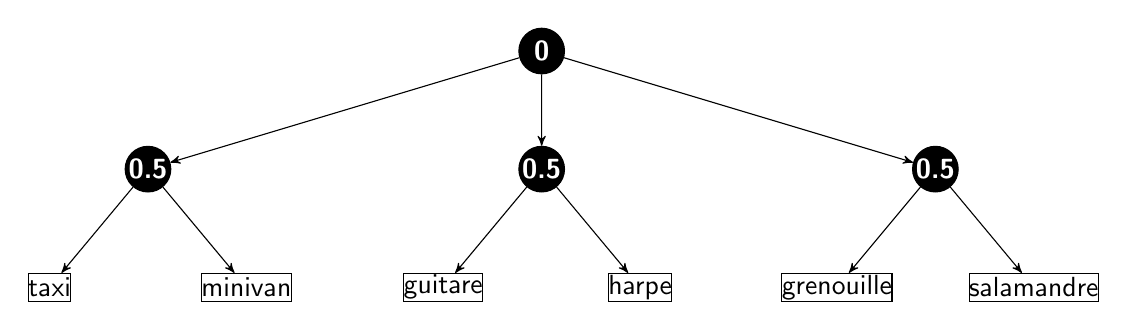
\begin{tikzpicture}[->,>=stealth',level/.style={sibling distance = 5cm/#1,
  level distance = 1.5cm}] 
\node [arn_n] {0}
    child{ node [arn_n] {0.5} 
            child{ node [arn_x] {taxi} 
            }
            child{ node [arn_x] {minivan}
            }
    }
     child{ node [arn_n] {0.5} 
            child{ node [arn_x] {guitare} 
            }
            child{ node [arn_x] {harpe}
            }
    }
    child{ node [arn_n] {0.5}
            child{ node [arn_x] {grenouille} 
            }
            child{ node [arn_x] {salamandre}
            }
		}
; 
\end{tikzpicture}

\subsection{Inteprétation des résultats}

\begin{figure}
\centering
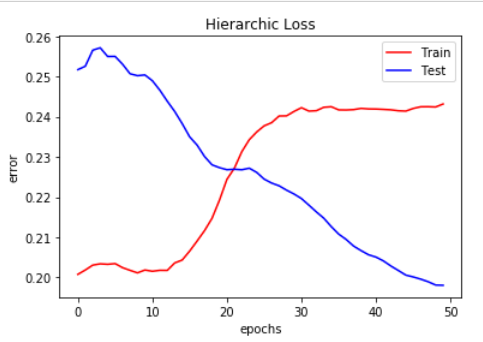
\includegraphics[width=0.75\textwidth]{HierLoss.png}
\caption{\label{fig:data} Évaluation de la Hierarchic loss en train et en test sur 100 epochs.}
\end{figure}

\begin{figure}
\centering
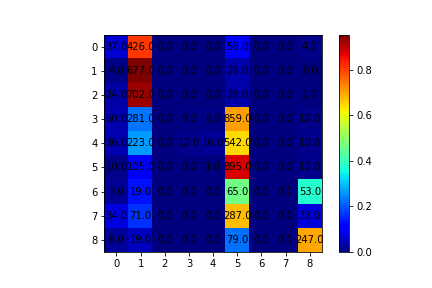
\includegraphics[width=1\textwidth]{confusionHier.png}
\caption{\label{fig:data} Matrice de confusion pour un modèle entrainé avec une Hierarchic loss sur 100 epochs. 0 = taxi, 1 = ambulance, 2 = minivan, 3 = acoustic guitar, 4 = electric guitar, 5 = harp, 6 = wood frog, 7 = tree frog, 8 = european fire salamander}
\end{figure}


\section{Apprentissage structuré appliqué au problème de ranking }
Dans cette seconde partie on s'intéresse à la résolution d'un problème d'ordonnancement grâce à l'apprentissage structuré.
\subsection{Ranking}
On définit cette fois notre espace d'entrée $X$ comme étant l'ensemble des représentations des images de notre ensemble de données sous forme de vecteurs de descriptions (\textit{Bag of Words}). On définit l'espace de sortie structuré $Y$ comme étant une liste d'ordonnancement des images par rapport à une requête.
Pour ce problème de ranking, on considère un étiquetage binaire des données. Dans ce cas on définit la \textit{joint feature map} et la fonction de coût de la façon suivante : 
\begin{equation}
\Psi(x,y) = \sum\limits_{i \in \oplus}  \sum\limits_{j \in \ominus} y_{ij} (\phi(x_i) - \phi(x_j))
\end{equation}
\begin{equation}
\Delta(y_i,y) = 1 - AP(y)
\end{equation}
Où 
\begin{itemize}
\item $\oplus$ représente l'ensemble des images placées avant l'ensemble $\ominus$ dans l'ordonnancement $y$
\item AP représente l'aire sous la courbe de précision/rappel (Précision Moyenne)
\end{itemize}


\subsection{Évaluation et inteprétation des résultats}

\section{Conclusion}


\end{document}